\section{CChanged\-Predicate$<$ T $>$  Class Template Reference}
\label{classCChangedPredicate}\index{CChangedPredicate@{CChanged\-Predicate}}
{\tt \#include $<$CChanged\-Predicate.h$>$}

Inheritance diagram for CChanged\-Predicate$<$ T $>$::\begin{figure}[H]
\begin{center}
\leavevmode
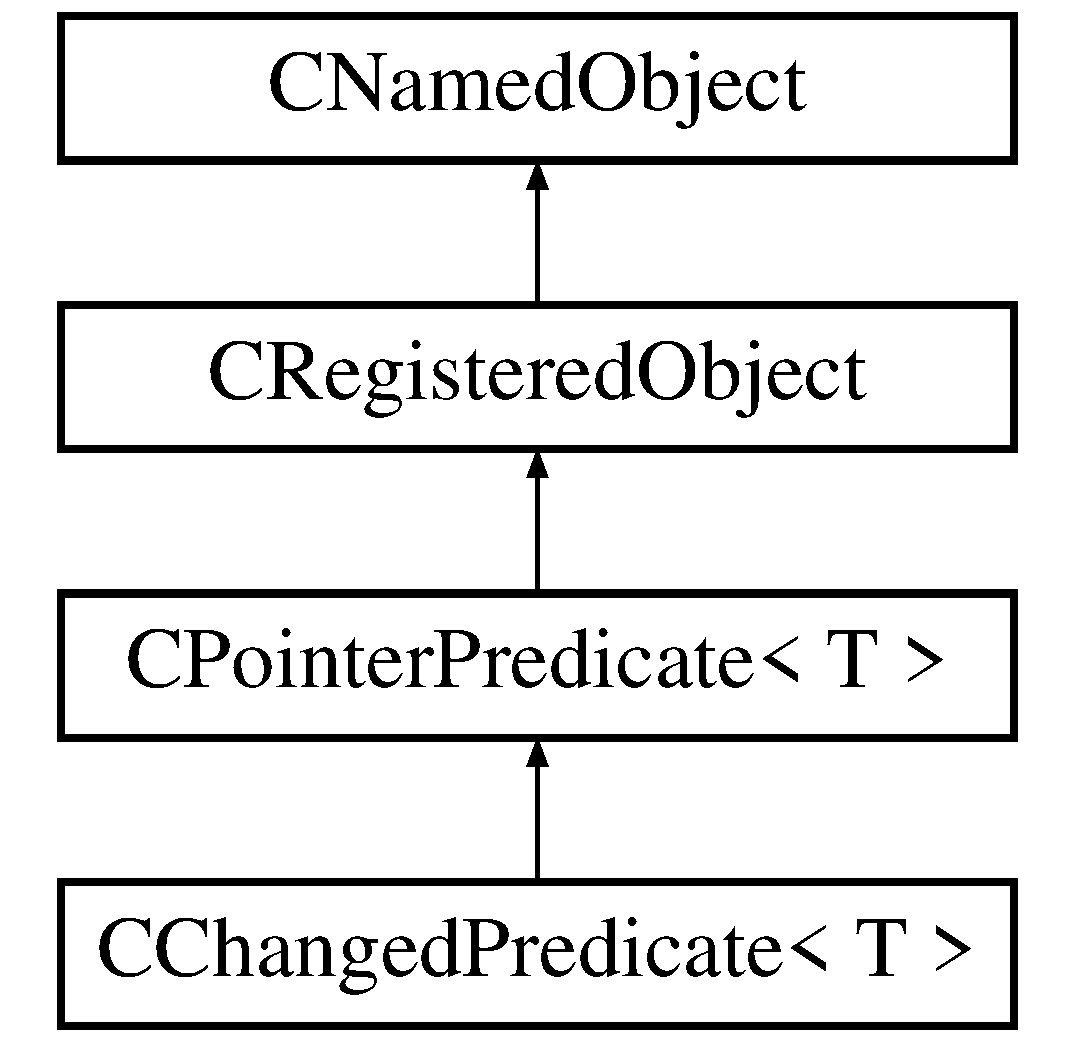
\includegraphics[height=4cm]{classCChangedPredicate}
\end{center}
\end{figure}
\subsection*{Public Methods}
\begin{CompactItemize}
\item 
{\bf CChanged\-Predicate} (T am\_\-TOld\-Value)
\item 
{\bf CChanged\-Predicate} (const string \&r\-Name, T am\_\-TOld\-Value)
\item 
{\bf CChanged\-Predicate} (const char $\ast$p\-Name, T am\_\-TOld\-Value)
\item 
{\bf $\sim$CChanged\-Predicate} ()
\item 
int {\bf operator==} (const CChanged\-Predicate$<$ T $>$ \&a\-CChanged\-Predicate) const
\item 
T {\bf get\-Old\-Value} () const
\item 
virtual bool {\bf operator()} (T n\-Value)
\item 
virtual string {\bf Describe\-Self} ()
\end{CompactItemize}
\subsection*{Protected Methods}
\begin{CompactItemize}
\item 
void {\bf set\-Old\-Value} (const T am\_\-TOld\-Value)
\end{CompactItemize}
\subsection*{Private Methods}
\begin{CompactItemize}
\item 
{\bf CChanged\-Predicate} (const CChanged\-Predicate$<$ T $>$ \&a\-CChanged\-Predicate)
\item 
CChanged\-Predicate$<$ T $>$ {\bf operator=} (const CChanged\-Predicate$<$ T $>$ \&a\-CChanged\-Predicate)
\end{CompactItemize}
\subsection*{Private Attributes}
\begin{CompactItemize}
\item 
T {\bf m\_\-TOld\-Value}
\end{CompactItemize}


\subsection{Detailed Description}
\subsubsection*{template$<$typename T$>$ class CChanged\-Predicate$<$ T $>$}

$\backslash$class: CChanged\-Predicate

Defines a pointer predicate which is satisfied whenever the current value changes.

Author: Jason Venema NSCL Michigan State University East Lansing, MI 48824-1321 mailto: {\tt venemaja@msu.edu} 



Definition at line 301 of file CChanged\-Predicate.h.

\subsection{Constructor \& Destructor Documentation}
\index{CChangedPredicate@{CChanged\-Predicate}!CChangedPredicate@{CChangedPredicate}}
\index{CChangedPredicate@{CChangedPredicate}!CChangedPredicate@{CChanged\-Predicate}}
\subsubsection{\setlength{\rightskip}{0pt plus 5cm}template$<$typename T$>$ CChanged\-Predicate$<$ T $>$::CChanged\-Predicate (T {\em am\_\-TOld\-Value})\hspace{0.3cm}{\tt  [inline]}}\label{classCChangedPredicate_a0}


Prior value \index{CChangedPredicate@{CChanged\-Predicate}!CChangedPredicate@{CChangedPredicate}}
\index{CChangedPredicate@{CChangedPredicate}!CChangedPredicate@{CChanged\-Predicate}}
\subsubsection{\setlength{\rightskip}{0pt plus 5cm}template$<$typename T$>$ CChanged\-Predicate$<$ T $>$::CChanged\-Predicate (const string \& {\em r\-Name}, T {\em am\_\-TOld\-Value})\hspace{0.3cm}{\tt  [inline]}}\label{classCChangedPredicate_a1}


\index{CChangedPredicate@{CChanged\-Predicate}!CChangedPredicate@{CChangedPredicate}}
\index{CChangedPredicate@{CChangedPredicate}!CChangedPredicate@{CChanged\-Predicate}}
\subsubsection{\setlength{\rightskip}{0pt plus 5cm}template$<$typename T$>$ CChanged\-Predicate$<$ T $>$::CChanged\-Predicate (const char $\ast$ {\em p\-Name}, T {\em am\_\-TOld\-Value})\hspace{0.3cm}{\tt  [inline]}}\label{classCChangedPredicate_a2}


\index{CChangedPredicate@{CChanged\-Predicate}!~CChangedPredicate@{$\sim$CChangedPredicate}}
\index{~CChangedPredicate@{$\sim$CChangedPredicate}!CChangedPredicate@{CChanged\-Predicate}}
\subsubsection{\setlength{\rightskip}{0pt plus 5cm}template$<$typename T$>$ CChanged\-Predicate$<$ T $>$::$\sim$CChanged\-Predicate ()\hspace{0.3cm}{\tt  [inline]}}\label{classCChangedPredicate_a3}


\index{CChangedPredicate@{CChanged\-Predicate}!CChangedPredicate@{CChangedPredicate}}
\index{CChangedPredicate@{CChangedPredicate}!CChangedPredicate@{CChanged\-Predicate}}
\subsubsection{\setlength{\rightskip}{0pt plus 5cm}template$<$typename T$>$ CChanged\-Predicate$<$ T $>$::CChanged\-Predicate (const CChanged\-Predicate$<$ T $>$ \& {\em a\-CChanged\-Predicate})\hspace{0.3cm}{\tt  [private]}}\label{classCChangedPredicate_c0}




\subsection{Member Function Documentation}
\index{CChangedPredicate@{CChanged\-Predicate}!DescribeSelf@{DescribeSelf}}
\index{DescribeSelf@{DescribeSelf}!CChangedPredicate@{CChanged\-Predicate}}
\subsubsection{\setlength{\rightskip}{0pt plus 5cm}template$<$typename T$>$ string CChanged\-Predicate$<$ T $>$::Describe\-Self ()\hspace{0.3cm}{\tt  [virtual]}}\label{classCChangedPredicate_a7}


Describes the named object. The information given is the object type given by m\_\-s\-Class\-Path, and the object name. 

Implements {\bf CPointer\-Predicate$<$ T $>$} {\rm (p.\,\pageref{classCPointerPredicate_a6})}.

Definition at line 319 of file CChanged\-Predicate.cpp.

References CChanged\-Predicate$<$ T $>$::m\_\-TOld\-Value.\index{CChangedPredicate@{CChanged\-Predicate}!getOldValue@{getOldValue}}
\index{getOldValue@{getOldValue}!CChangedPredicate@{CChanged\-Predicate}}
\subsubsection{\setlength{\rightskip}{0pt plus 5cm}template$<$typename T$>$ T CChanged\-Predicate$<$ T $>$::get\-Old\-Value () const\hspace{0.3cm}{\tt  [inline]}}\label{classCChangedPredicate_a5}




Definition at line 344 of file CChanged\-Predicate.h.\index{CChangedPredicate@{CChanged\-Predicate}!operator()@{operator()}}
\index{operator()@{operator()}!CChangedPredicate@{CChanged\-Predicate}}
\subsubsection{\setlength{\rightskip}{0pt plus 5cm}template$<$typename T$>$ bool CChanged\-Predicate$<$ T $>$::operator() (T {\em n\-Value})\hspace{0.3cm}{\tt  [virtual]}}\label{classCChangedPredicate_a6}




Implements {\bf CPointer\-Predicate$<$ T $>$} {\rm (p.\,\pageref{classCPointerPredicate_a5})}.

Definition at line 300 of file CChanged\-Predicate.cpp.

References CChanged\-Predicate$<$ T $>$::m\_\-TOld\-Value.\index{CChangedPredicate@{CChanged\-Predicate}!operator=@{operator=}}
\index{operator=@{operator=}!CChangedPredicate@{CChanged\-Predicate}}
\subsubsection{\setlength{\rightskip}{0pt plus 5cm}template$<$typename T$>$ CChanged\-Predicate$<$T$>$ CChanged\-Predicate$<$ T $>$::operator= (const CChanged\-Predicate$<$ T $>$ \& {\em a\-CChanged\-Predicate})\hspace{0.3cm}{\tt  [private]}}\label{classCChangedPredicate_c1}


\index{CChangedPredicate@{CChanged\-Predicate}!operator==@{operator==}}
\index{operator==@{operator==}!CChangedPredicate@{CChanged\-Predicate}}
\subsubsection{\setlength{\rightskip}{0pt plus 5cm}template$<$typename T$>$ int CChanged\-Predicate$<$ T $>$::operator== (const CChanged\-Predicate$<$ T $>$ \& {\em a\-CChanged\-Predicate}) const\hspace{0.3cm}{\tt  [inline]}}\label{classCChangedPredicate_a4}




Definition at line 327 of file CChanged\-Predicate.h.

References CChanged\-Predicate$<$ T $>$::m\_\-TOld\-Value, and CPointer\-Predicate$<$ T $>$::operator==().\index{CChangedPredicate@{CChanged\-Predicate}!setOldValue@{setOldValue}}
\index{setOldValue@{setOldValue}!CChangedPredicate@{CChanged\-Predicate}}
\subsubsection{\setlength{\rightskip}{0pt plus 5cm}template$<$typename T$>$ void CChanged\-Predicate$<$ T $>$::set\-Old\-Value (const T {\em am\_\-TOld\-Value})\hspace{0.3cm}{\tt  [inline, protected]}}\label{classCChangedPredicate_b0}




Definition at line 352 of file CChanged\-Predicate.h.

\subsection{Member Data Documentation}
\index{CChangedPredicate@{CChanged\-Predicate}!m_TOldValue@{m\_\-TOldValue}}
\index{m_TOldValue@{m\_\-TOldValue}!CChangedPredicate@{CChanged\-Predicate}}
\subsubsection{\setlength{\rightskip}{0pt plus 5cm}template$<$typename T$>$ T CChanged\-Predicate$<$ T $>$::m\_\-TOld\-Value\hspace{0.3cm}{\tt  [private]}}\label{classCChangedPredicate_o0}




Definition at line 303 of file CChanged\-Predicate.h.

Referenced by CChanged\-Predicate$<$ T $>$::Describe\-Self(), CChanged\-Predicate$<$ T $>$::operator()(), and CChanged\-Predicate$<$ T $>$::operator==().

The documentation for this class was generated from the following files:\begin{CompactItemize}
\item 
{\bf CChanged\-Predicate.h}\item 
{\bf CChanged\-Predicate.cpp}\end{CompactItemize}
